\documentclass[a4paper, 12pt]{article}

\usepackage[margin=2.5cm]{geometry}

\usepackage{graphicx}
\usepackage[export]{adjustbox}

\usepackage{anyfontsize}
\usepackage{titlesec}
\usepackage{setspace}
\usepackage{parskip}

\usepackage[table]{xcolor}
\usepackage{makecell}

\usepackage{listings}

\usepackage{amsmath}
\usepackage{pgfplots}
\pgfplotsset{compat = newest}

\usepackage{pdfpages}

\usepackage{hyperref}
\hypersetup{
    colorlinks,
    citecolor=black,
    filecolor=black,
    linkcolor=black,
    urlcolor=black
}
% causes warning because hyperref doesn't like hebrew

\usepackage{polyglossia}
\setmainlanguage{hebrew}
\setotherlanguage{english}
\setmonofont{FreeSerif}
\newfontfamily{\englishfont}{David Libre}
\newfontfamily{\englishfontcode}{JetBrainsMono-Regular}
\newfontfamily{\hebrewfont}{David Libre}

% \begin{english}
% this is where english text can be inserted
% \end{english}

% can also use \textenglish{english text goes here}

% Font - David
% Normal Size - 12pt
% Spacing - 1.15
% Section Size - 16pt
% Subsection Size - 14pt

\titleformat*{\section}{\fontsize{16}{19.2}\selectfont\bfseries}
\titleformat*{\subsection}{\fontsize{14}{16.8}\selectfont\bfseries}
\titleformat*{\subsubsection}{\fontsize{12}{14.4}\selectfont\bfseries}

\setlength{\parindent}{0pt} % removes default paragraph indentation
\setstretch{1.15} % spacing
\setcounter{secnumdepth}{0} % doesn't number sections
\setcounter{tocdepth}{1} % depth of ToC (will only show parts, chapters, sections)


\title{דוח מעבדה \\ תנועת הירחים של צדק}
\author{אביאל וויסמן \\ \small{דרכא בית ירח}}
\date{2023 \\ ינואר}

% ----- Report ----- %

\begin{document}
    
    \maketitle

    \vfill

    \hrule
    \vspace{15pt}

    \renewcommand{\abstractname}{מטרת הניסוי}
    \begin{abstract}
        \centering
        מטרת הניסוי היא למדוד את מסלוליהם של הירחים של צדק ולהשתמש בחוק השלישי של קפלר כדי למצוא את מסת צדק.
    \end{abstract}

    \vspace{15pt}
    \hrule

    \vfill

    {\makeatletter
        \def\@@underline#1{#1}
        \tableofcontents
    \makeatother} % doesn't underline sections in the ToC

    \vfill

    \pagebreak % ----- Page Break ----- %

    \section{\underline{רקע תיאורטי}}

    \begin{flushright}
        לצורך ניסוי זה אנו מניחים שזמן ורדיוס המסלול של ירח סביב 
        צדק נשאר קבוע.
        בנוסף אנחנו גם מניחים שירח מקיף את צדק במסלול מעגלי (למרות שבמציאות זה אליפטי).
    \end{flushright}

    \begin{figure}[h!]
        \centering
        \begin{minipage}{0.4\textwidth}
            \centering
            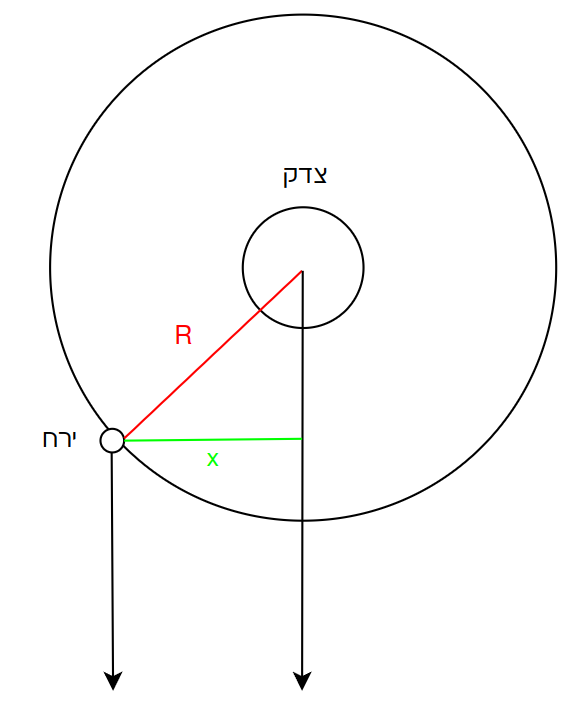
\includegraphics[width=0.8\textwidth]{../assets/orbit_from_above_01.png}
        \end{minipage}\hfill
        \begin{minipage}{0.55\textwidth}
            \centering
            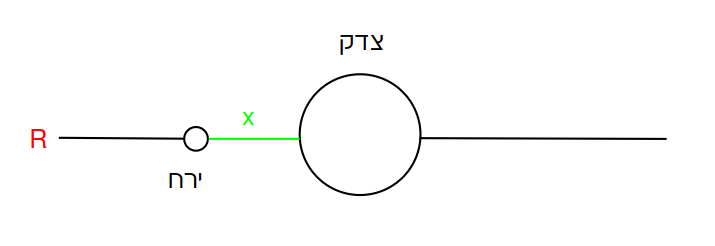
\includegraphics[width=\textwidth]{../assets/orbit_from_earth_01.png}
        \end{minipage}
        \caption{מבט מלמעלה ומכדור הארץ}
        \label{orbit_01}
    \end{figure}

    \begin{figure}[h!]
        \centering
        \begin{minipage}{0.4\textwidth}
            \centering
            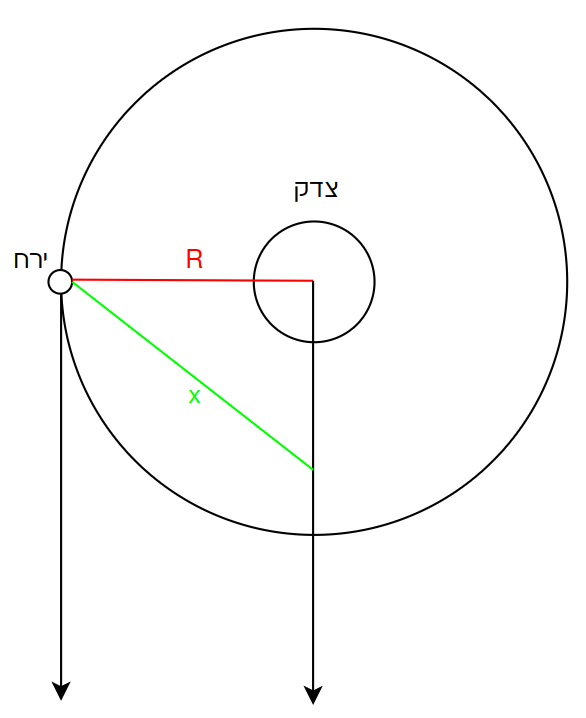
\includegraphics[width=0.8\textwidth]{../assets/orbit_from_above_02.png}
        \end{minipage}\hfill
        \begin{minipage}{0.55\textwidth}
            \centering
            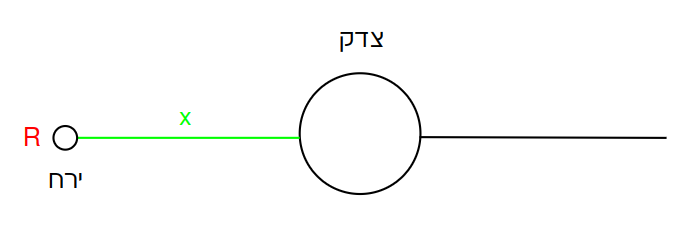
\includegraphics[width=\textwidth]{../assets/orbit_from_earth_02.png}
        \end{minipage}
        \caption{מבט מלמעלה ומכדור הארץ}
        \label{orbit_02}
    \end{figure}

    \begin{flushright}
        ניתן לראות ש \textcolor{green}{x} הוא המרחק הנראה של ירח מצדק,
        מנקודת מבטנו מכדור הארץ, ו \textcolor{red}{R} הוא רדיוס המסלול של ירח סביב צדק.

        מנקודת מבט מכדור הארץ הירח נע על ציר אחד (ציר אופקי), כלומר
        כפי שנראה מכדור הארץ, הירח ינוע ימינה ושמאלה.
        דבר זה מתרחש מכיוון שאנחנו (כדור הארץ) וצדק נמצאים על אותו מישור במסלול שלנו סביב השמש.
        
        בעזרת טריגונומטריה אפשר לחשב את \textcolor{green}{x} המרחק הנראה של הירח מצדק,
        יוצא ש
        $ x = Rsin{\alpha} $.
        בעקבות זאת אנחנו נצפה לראות פונקציה סינוסואידלית עבור המרחק של הירח מצדק 
        מנקודת מבטנו.
    \end{flushright}

    \pagebreak % ----- Page Break ----- %

    \subsection{בניית המשוואות }

    \begin{flushright}
        אנחנו נבנה
        משוואת כוחות עבור ירח שמסתו $m$ שנע במסלול מעגלי סביב גוף מסיבי שמסתו $M$ (במקרה זה הוא צדק):
        
        נעזר בחוק השני של ניוטון.

        $$ \Sigma \vec{F} = m\vec{a} $$ 

        במקרה זה פועל רק כוח הכבידה, ומיכוון שהירח מקיף את הגוף המסיבי בצורה מעגלית
        קיים תאוצה רדיאלית (צנטריפטלית). 

        $$ F_G = ma_r $$

        אנחנו נחליף את $F_G$ ו $a_r$ במשוואות שלהם, ונציב בהם את המשתנים שלנו.

        $$ G\dfrac{mM}{R^2} = m \omega^2 R$$

        אנחנו נחליף את התדירות הזוויתית $\omega$ במשוואה שלה ונפשט.
        
        $$ \dfrac{GmM}{R^2} = m \biggl(\dfrac{2\pi}{T}\biggl)^2 R $$
        
        $$ \dfrac{GM}{R^2} = \dfrac{4\pi^2}{T^2} R $$
    \end{flushright}

    \begin{english}
        \begin{equation}
            \label{firsteq}
            \dfrac{GM}{4\pi^2} = \dfrac{R^3}{T^2}
        \end{equation}
    \end{english}

    \begin{flushright}
        אנחנו נבנה
        משוואת כוחות עבור כדור הארץ שמקיף את השמש שמסתה $M_S$ במסלול שרידוסו
        $R_E$ בזמן הקפה $T_E$:

        אנחנו נציב משתנים אלו \textbf{במשוואה \ref{firsteq}} למעלה, ונקבל:
    \end{flushright}

    \begin{english}
        \begin{equation}
            \label{secondeq}
            \dfrac{GM_S}{4\pi^2} = \dfrac{R_E^3}{T_E^2}
        \end{equation}
    \end{english}

    \pagebreak % ----- Page Break ----- %

    \begin{flushright}
        נחלק \textbf{משוואה \ref{firsteq} ב- \ref{secondeq}}:
    \end{flushright}

    \begin{align*}
        \dfrac{\dfrac{GM}{4\pi^2}}{\dfrac{GM_S}{4\pi^2}} 
        = \dfrac{\dfrac{R^3}{T^2}}{\dfrac{R_E^3}{T_E^2}} 
        \quad\Rightarrow\quad
        \dfrac{M}{M_S} &= \dfrac{R^3}{T^2} \times \dfrac{T_E^2}{R_E^3} &\text{נחלק שבר בשבר והחלפה בין המכנים} \\[0.5em]
        \dfrac{M}{M_S} &= \dfrac{R^3}{R_E^3} \times \dfrac{T_E^2}{T^2} &\text{נעביר מכפל לחילוק בין השברים} \\[0.5em]
        \dfrac{M}{M_S} &= \dfrac{\dfrac{R^3}{R_E^3}}{\dfrac{T^2}{T_E^2}} &\text{נשתמש בחוקי חזקות}
    \end{align*}
    
    \begin{english}
        \begin{equation}
            \label{thirdeq}
            \dfrac{M}{M_S} = \dfrac{\biggl(\dfrac{R}{R_E}\biggl)^3}{\biggl(\dfrac{T}{T_E}\biggl)^2} 
        \end{equation}
    \end{english}
        
    \begin{flushright}
        קיבלנו משוואה המתארת את הקשר בין מסת גוף מסיבי (ביחידות מסת שמש)
        לבין היחס של רדיוס מסלולו (ביחידות אסטרונומיות \textenglish{AU}\footnotemark{}( לזמן המחזור של הקפתו (בשנים).

        בניסוי זה אנחנו נחשב את מסת צדק ביחידות מסת שמש. נעשה זאת באמצעות
        הוצאת מידע מהניסוי על רדיוס וזמן מחזור של ירח סביב צדק.

        בהדמיה משתמשים ביחידות שונות לאלו שאנחנו משתמשים בהם \textbf{במשוואה \ref{thirdeq}}, לכן נמיר יחידות אלו.
        בהדמיה משתמשים ביחידות של קטרי צדק (פעמיים רדיוס צדק) עבור רדיוס המסלול
        ויחידות ימים עבור זמן המחזור של ההקפה, 
        נמיר אותם ליחידות
        \textenglish{AU} ושנים בהתאמה:
        $$ \dfrac{AU}{\text{\texthebrew{קוטר צדק}}} = \dfrac{149.6\times10^9}{2\times71.4\times10^6} = 1047 m $$
        $$ \dfrac{\text{שנים}}{\text{ימים}} = 365 $$

        מחישובים אלו נובע שצריך לחלק את תוצאות הרדיוס מהניסוי ב-1047 כדי שיהיו ביחידות \textenglish{AU},
        ושצריך לחלק את תוצאות הזמן מחזור מהניסוי ב-365 כדי שיהיו ביחידות שנים.
    \end{flushright}
    
    \vfill

    \footnotetext{מרחק ממוצע מכדור הארץ לשמש, כלומר רדיוס ההקפה של כדור הארץ סביב השמש.}

    \pagebreak % ----- Page Break ----- %

    \section{\underline{מערכת הניסוי}}
    \begin{flushright}
        במעבדה זו נשתמש במחשב להדמית תצפית על ארבעת הירחים של צדק,
        אנחנו נצפה בארבעת הירחים הגליליאניים - איו, אירופה, גנימד, קליסטו.

        על מנת שיהיה קל יותר לזהות את הירחים ניתן לתת לכל ירח צבע אחר, נעשה זאת כך:\\
        \textenglish{File $\rightarrow$ Preferences $\rightarrow$ ID Colors}.
    \end{flushright}

    \vspace{40pt}

    \begin{figure}[h!]
        \centering
        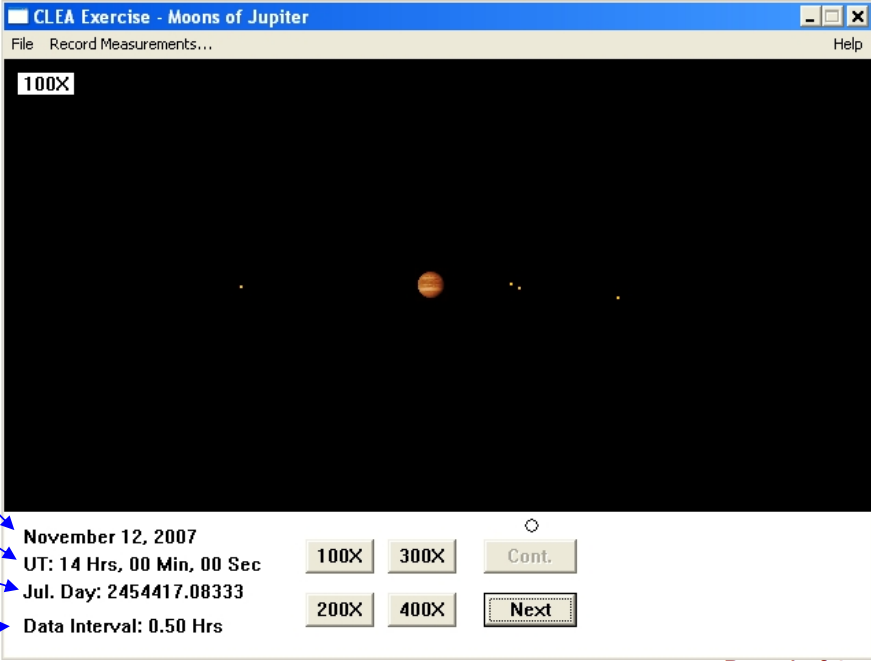
\includegraphics[width=\textwidth]{../assets/software_image.png}
        \caption{תוכנת הדמיית המחשב}
    \end{figure}

    \pagebreak % ----- Page Break ----- %

    \section{\underline{מהלך הניסוי}}
    \begin{flushright}
        במהלך הניסוי נבצע את אותם השלבים על כל ירח:

        \begin{enumerate}
            \item[.1] נקבע את מרווחי הזמן בין כל תצפית בצורה הבאה:
            \begin{itemize}
                \item איו - 2 שעות
                \item אירופה - 4 שעות
                \item גנימד - 6 שעות
                \item קליסטו - 8 שעות
            \end{itemize}
            נעשה זאת כך: \textenglish{File $\rightarrow$ Preferences $\rightarrow$ Timing}, לשנות את הערך של 
            \textenglish{Observation Interval}.
            
            \item[.2] נמדוד את המיקום של כל ירח
            נעשה זאת על ידי לחיצה שמאלית על הירח באצעות העכבר, בפינה הימנית התחתונה של המסך
            יופיע מידע על הירח שלחצנו על, מידע זה כולל: שם הירח, מיקום על המסך, המרחק מצדק
            ובאיזה צד \textenglish{(W או E)} הירח נראה לעומת צדק.
            אם שם הירח אינו מופיע שם, יש לדייק בלחיצת העכבר על הירח, מומלץ מאוד להשתמש
            בהגדלה הכי גדולה שעבורה הירח אינו חורג מגבולות המסך.
            
            כאשר אנחנו מרוצים מהמדידה, אנו צריכים ללחוץ על
            Record כדי שהמידע יקלט לתוכנה.
            ניתן להוסיף או לערוך נתונים על ידי \textenglish{File $\rightarrow$ Data $\rightarrow$ Review}.
            
            בסוף מדידה יש ללחוץ על כפתור \textenglish{Next}. 
            יש לבצע בין 30-20 מדידות לכל ירח על מנת לקבל מספיק דגימות
            כדי ליצור פונקציה של מסלול כל ירח סביב צדק. לאורך הניסוי יהיו תצפיות שלא ניתן למדוד בהן, במקרה זה
            נדלג לתצפית הבאה מבלי למדוד.
        \end{enumerate}
    \end{flushright}

    \section{\underline{תוצאות הניסוי}}
    \begin{flushright}
        האפשרות לבנות גרף סינוס מובנית בתוכנה, נעשה זאת כך:
        \begin{enumerate}
            \item[.1] נבחר איזה ירח אנחנו רוצים ליצור לו גרף, נעשה זאת כך: 
            \textenglish{File $\rightarrow$ Data $\rightarrow$ Analyze} ואז נבחר ירח.
            לאחר מכן נבחר \textenglish{Plot $\rightarrow$ Plot Type $\rightarrow$ Show Points}.
            \item[.2] נקבע זמן מחזור של הפונקציה, נעשה זאת על ידי לחיצה שמאלית על נקודה שבה 
            הגרף אמור לחצות את ציר הזמן, בחר כעת
            \textenglish{Plot $\rightarrow$ Fit Sine Curve $\rightarrow$ Set Initial Parameters},
            ונזין את הזמן שמצאנו בתור \textenglish{T-Zero}.
            אנחנו נחזור על הפעולה הזו שוב עבור נקודה סמוכה שבה הגרף אמור לחתוך את ציר הזמן,
            נחשב את זמן המחזור ונציב זמן זה בתור \textenglish{Period}.
            \item[.3] באופן דומה לסעיף הקודם, יש למצוא את המשרעת של הפונקציה.
            \item[.4] לאחר הזנת כל נתוני פונקצית הסינוס, נלחץ על \textenglish{OK} ויופיע גרך סינוס.
            במידה שהגרף אינו עובר דרך כל הנקודות, עלינו לחזור על השלבים הקודמים. אם רק כמה נקודות
            חורגות מעקומת הסינוס, הדבר נובע כנראה מאי-דיוק במדידה.
            ניתן להשתמש בשלושת פסי הגלילה כדי לשפר את ההתאמה של עקומת הסינוס לנקודות.

            יש לשאוף לערך \textenglish{RMS Residual} מינימלי.
        \end{enumerate}
    \end{flushright}


    \pagebreak % ----- Page Break ----- %

    \begin{figure}[h!]
        \centering
        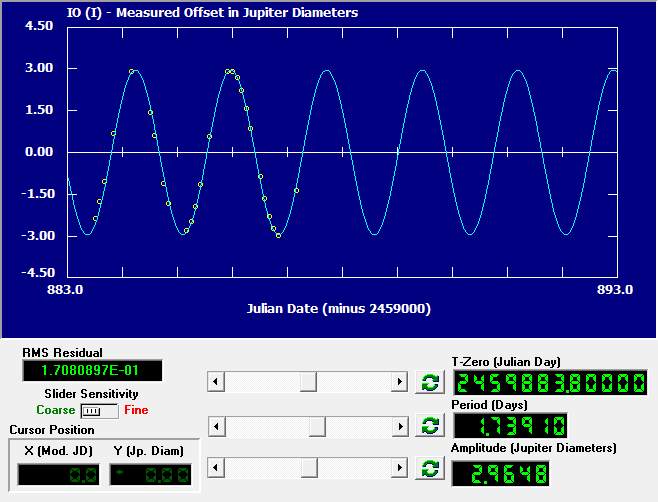
\includegraphics[width=0.8\textwidth]{../assets/io_graph.png}
        \caption{איו}
    \end{figure}

    \vfill

    \begin{figure}[h!]
        \centering
        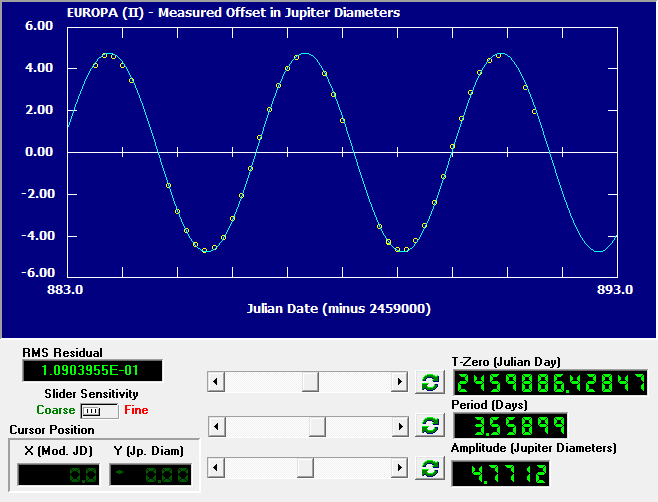
\includegraphics[width=0.8\textwidth]{../assets/europa_graph.png}
        \caption{אירופה}
    \end{figure}

    \vfill

    \pagebreak % ----- Page Break ----- %

    \begin{figure}[h!]
        \centering
        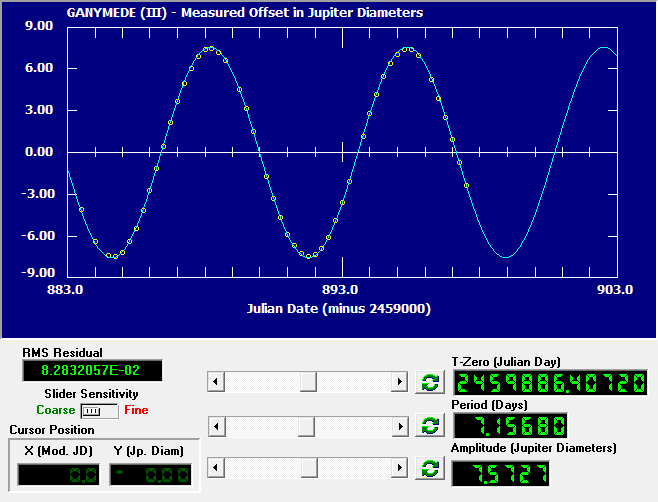
\includegraphics[width=0.8\textwidth]{../assets/ganymede_graph.png}
        \caption{גנימד}
    \end{figure}

    \vfill

    \begin{figure}[h!]
        \centering
        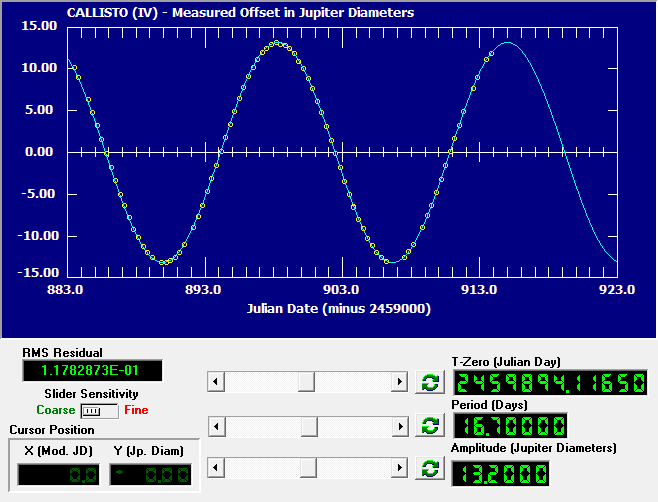
\includegraphics[width=0.8\textwidth]{../assets/callisto_graph.png}
        \caption{קליסטו}
    \end{figure}

    \vfill

    \pagebreak % ----- Page Break ----- %

    \section{\underline{עיבוד וניתוח תוצאות}}
    \begin{flushright}
        ניתן לראות בתמונות של התוצאות שלנו שהציר האופקי
        מסמל את הזמן ביחידות ימים, ושהציר האנכי מסמל המרחק הנראה של ירח מצדק (מנקודת מבט מכדור הארץ)
        ביחידות קוטרי צדק.

        האמפליטודה מסמלת את רדיוס המסלול של ירח סביב צדק, זהו המרחק הנראה המקסימלי של ירח מצדק.
        ניתן להסתכל על \textbf{איור \ref{orbit_02}} ולראות שכאשר הירח נמצא בזווית 
        \textenglish{$90^\circ$} או \textenglish{$270^\circ$} 
        המרחק הנראה הוא למעשה רדיוס ההקפה. ניתן להראות זאת באופן מתמטי בעזרת הביטוי
        $( x = R\sin{\alpha} )$
        שמצאנו לחישוב מרחק נראה של ירח מצדק.

        $$ x = R\sin{90^\circ} = R\times 1 \quad \Rightarrow \quad x = R $$
        $$ x = R\sin{270^\circ} = R\times -1 \quad \Rightarrow \quad x = -R $$
    \end{flushright}

    \vspace{15pt}

    \begin{flushright}
        אנחנו נכניס לטבלה מידע על אמפליטודה (רדיוס מסלול) וזמן מחזור של כל ירח מתוצאות שלנו,
        אנחנו נעגל לספרה השנייה אחרי הנקודה.
    \end{flushright}

    \vspace{10pt}

    \begin{table}[h!]
        \centering
        \setlength{\tabcolsep}{10pt} % Default value: 6pt
        \begin{tabular}{ c c c }
            ירח & \makecell{אמפליטודה \\ (קטרי צדק)} & \makecell{זמן מחזור \\ (ימים)} \\
            \hline
            Io & 2.96 & 1.74 \\
            Europa & 4.77 & 3.56 \\ 
            Ganymede & 7.57 & 7.16 \\
            Callisto & 13.20 & 16.70 \\
        \end{tabular}
    \end{table}

    \vspace{10pt}

    \begin{flushright}
        אנחנו נמיר ליחידות מתאימות בעזרת החישובים שעשינו ברקע התיאורטי, כלומר
        נחלק את האמפליטודה ב1047 ואת זמן המחזור ב365 ונעגל את התוצאות
        לשלוש ספרות אחרי הנקודה.
    \end{flushright}

    \begin{table}[h!]
        \centering
        \setlength{\tabcolsep}{10pt} % Default value: 6pt
        \begin{tabular}{ c c c }
            ירח & \makecell{רדיוס מסלול \\ (AU)} & \makecell{זמן מחזור \\ (שנים)} \\
            \hline
            Io & 0.003 & 0.005 \\
            Europa & 0.005 & 0.01 \\ 
            Ganymede & 0.007 & 0.02 \\
            Callisto & 0.013 & 0.046 \\
        \end{tabular}
    \end{table}

    \vspace{10pt}

    \begin{flushright}
        אנחנו נעלה את הרדיוס בשלישית - $R^3$ ואת זמן המחזור בריבוע - $T^2$, מיכוון שאנחנו
        רוצים להשתמש \textbf{משוואה \ref{thirdeq}}.
    \end{flushright}

    \begin{table}[h!]
        \centering
        \setlength{\tabcolsep}{10pt} % Default value: 6pt
        \begin{tabular}{ c c c }
            ירח & \textenglish{$R^3$ (AU)} & \textenglish{{$T^2$} (שנים)} \\
            \hline
            Io & 0.000000027 & 0.000025 \\
            Europa & 0.000000125 & 0.0001 \\ 
            Ganymede & 0.000000343 & 0.0004 \\
            Callisto & 0.000002197 & 0.002116 \\
        \end{tabular}
    \end{table}

    \pagebreak % ----- Page Break ----- %

    \subsection{\underline{גרף של רדיוס מסלול לעומת זמן מחזור}}

    \begin{flushright}
        באמצעות המידע מהטבלה עם ערכי $R^3$ ו $T^2$ ביחידות AU ושנים בהתאמה,
        אנחנו ניצור גרף שמתארת את \textbf{משוואה \ref{thirdeq}}, במשוואה זו החילוק בין
        $R^3$ ל $T^2$ נותן את המסה של צדק.
        זאת אמרת שהשיפוע של הגרף שניצור יהיה המסה של צדק ביחידות מסת שמש.
    \end{flushright}

    \vspace{30pt}

    \begin{figure}[h!]
        \centering
        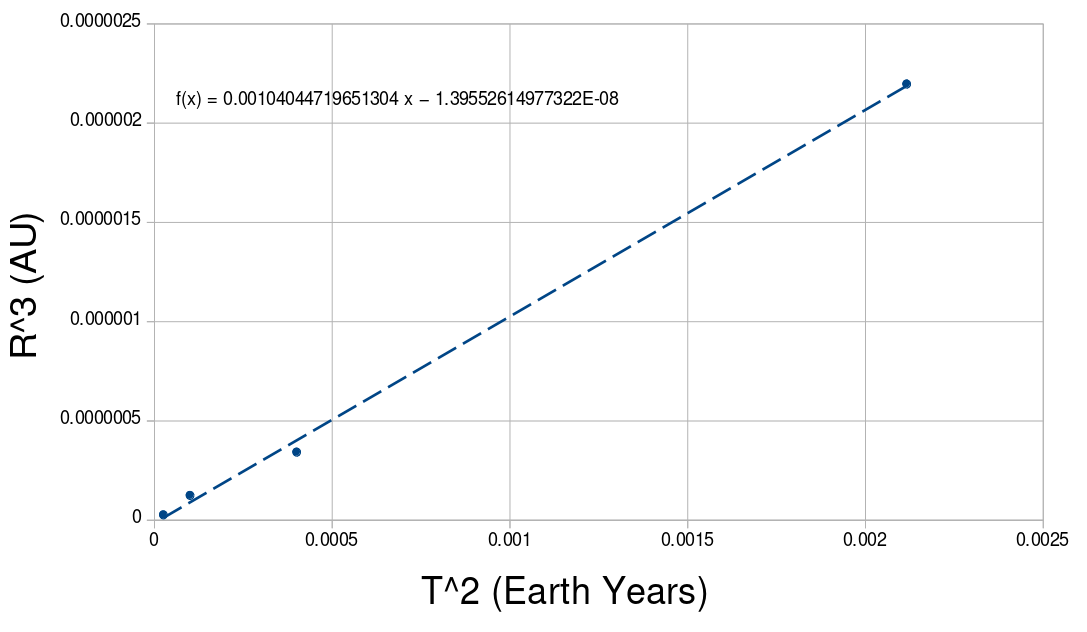
\includegraphics[width=\textwidth]{../assets/final_graph.png}
        \caption{גרף המבטא את החוק השלישי של קפלר}
    \end{figure}

    \vspace{30pt}

    \begin{flushright}
        ניתן לראות ששיפוע הגרף הוא כ \textenglish{0.001}, זאת אמרת שהיחס בין
        מסת צדק למסת השמש היא \textenglish{0.001}.

        $$ \dfrac{M_J}{M_S} = 0.001 $$

        אנחנו נציב את מסת השמש כדי למצוא את מסת צדק.

        $$ \dfrac{M_J}{1.99\times10^{30}} = 0.001 $$

        $$ M_J = 1.99\times10^{27} kg$$
    \end{flushright}


    \pagebreak % ----- Page Break ----- %

    \section{\underline{סיכום מסקנות}}
    \begin{flushright}
        לסיכום אנחנו מדדנו את מסלוליהם ירחי של צדק והשתמשנו במידע זה
        ובאמצעות החוק השלישי של קפלר כדי למצוא את היחס בין מסת צדק למסת השמש, ובכך
        למצוא את מסת צדק.

        המדידות נעשו ביחידות של קטרי צדק וימים ואנחנו היינו צריכים
        להמיר אותם ליחידות AU ושנים.
    \end{flushright}

\end{document}